
\section*{Learning Objectives}

\begin{itemize}
\item Learn about ``convexity'', which defines a class of problems where local minima are also global minima
\item Learn about two types of convex optimization problems that are fast enough to run in real time on many mobile platforms.
\end{itemize}

\section*{Outcomes} 
\begin{itemize}
\item  Definition of convex sets and convex functions.
\item Local minima of convex functions are also global minima.
\item A Quadratic Program (QP) is an optimization problem with a quadratic cost and linear inequality and equality constraints.
\item A Linear Program (LP) is an optimization problem with a linear cost and linear inequality and equality constraints.
\item Through the concept of ``slack variables'', an optimization problem with either a one-norm or $\infty$-norm as the the cost and linear inequality and equality constraints can be turned into an LP.
\end{itemize}

\newpage

\section{Brief Remarks on Convex Sets and Convex Functions}

\begin{definition}  Let $(\mathcal{X},\real)$ be a real vector space. $C \subset V$ is \textbf{ convex} if $\forall x,y \in C $ and $ 0\le \lambda \le 1$, the \textbf{convex combination} $\lambda x +(1-\lambda)y \in C$.

\end{definition}


\begin{rem} 
$$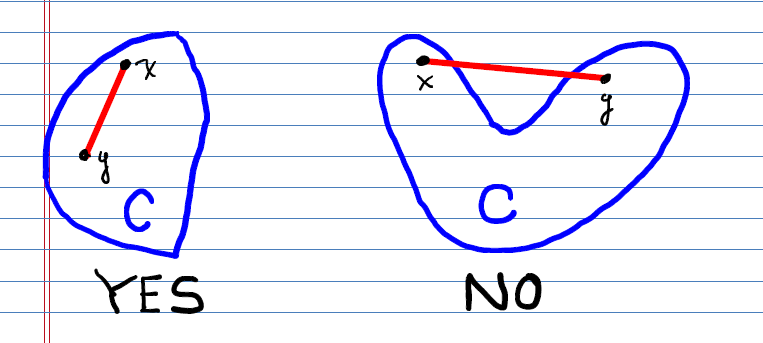
\includegraphics[width=0.70\columnwidth]{graphics/Chap06/ConvexSet.png} $$
\renewcommand{\labelenumi}{(\alph{enumi})}
\begin{enumerate}
\item For $C$ to be convex, given any two points $x,y \in C$, then the line connecting $x$ and $y$ must also lie in $C$.
\item Open and closed balls arsing from norms are always convex. 
\end{enumerate}
\end{rem}

\begin{definition} The \textbf{convex hull} of a set $S \subset \mathcal{X}$ is
$${\rm co}(S):=\{ \lambda x + (1 - \lambda)y ~|~ 0 \le \lambda \le 1, x, y \in S\}, $$
the set of all convex combinations of elements of $S$. It can also be defined as the smallest convex set that contains $S$. 
\end{definition}
$$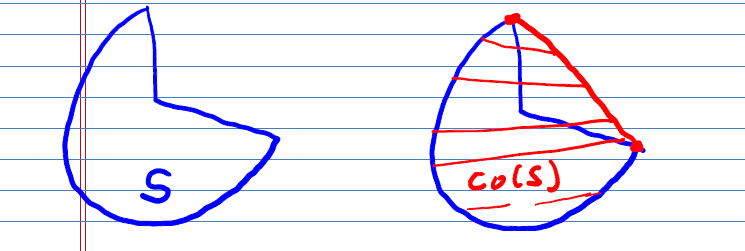
\includegraphics[width=0.70\columnwidth]{graphics/Chap06/ConvexHull.png} $$

\begin{definition} Suppose $C\subset \mathcal{X}$ is convex. A function
$f:C\to \real$ is \textbf{ convex} if $~\forall x,y \in C, 0 \le \lambda \le 1$,
$$f\left(\lambda x+(1-\lambda) y\right)\le \lambda f(x)+(1-\lambda)f(y).$$
\end{definition}
$$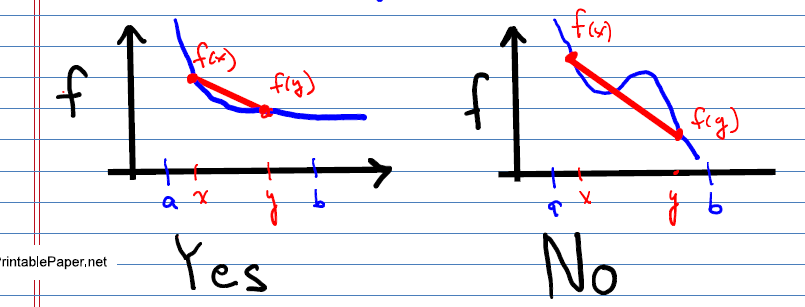
\includegraphics[width=0.70\columnwidth]{graphics/Chap06/ConvexFunction.png} $$

\begin{rem} For a function to be convex, the line $\lambda x + (1 - \lambda)y$ connecting $x$ and $y$ must lie at or above the graph of the function; it can never go below.

\end{rem}


\begin{definition} Suppose $(\mathcal{X},\real,||  \bullet ||)$ is a normed space, $D\subset \mathcal{X}$ a subset, and $f:D\to \real$ a function.
\renewcommand{\labelenumi}{(\alph{enumi})}
\begin{enumerate}
\item
$x^\ast \in D$ is a \textbf{ local minimum} of $f$ if $\exists \delta >0$ such that $\forall x\in B_\delta(x^\ast)$,
$f(x^\ast) \le f(x)$.
\item
$x^\ast \in D$ is a \textbf{ global minimum} if $\forall y \in D$, $f(x^\ast) \le f(y)$.
\end{enumerate}

\end{definition}

\begin{thm}\textbf{(Local equals Global for Convex Functions)} If $D$ and $f$ are both convex, then any local minimum is also a global minimum.
\end{thm} 

\textbf{ Proof:}~  We show that if $x$ is not a global minimum, then it cannot be a local minimum. Specifically, we prove the contrapositive statement: $((a) \implies (b)) \iff (\lnot (b) \implies \lnot (a))$, where
\begin{enumerate}
       \renewcommand{\labelenumi}{(\alph{enumi})}
        \setlength{\itemsep}{.1cm}
    \item $x\in D$ is a local minimum
    \item $x \in D$ is a global minimum.
       
    \item[$\lnot$(b)] $\exists y \in D$ such that $f(y) < f(x)$.
    
     \item[$\lnot$(a)] $\forall~\delta>0, \exists~z\in B_\delta(x) \cap D$ such that $f(z) < f(x)$.
\end{enumerate}

\begin{claim} If $f(y) < f(x)$, then $\forall  0<\lambda\le 1$, the vector  $z:=(1-\lambda)x+\lambda y$ satisfies $f(z) < f(x)$.
\end{claim}

Proof:  
\begin{align*}
        f(z)&=f((1-\lambda)x+\lambda y)\\
        &\le (1-\lambda)f(x)+\lambda f(y) ~~[\text{convexity}]\\
        &<(1-\lambda)f(x)+\lambda f(x)~~ [f(x) > f(y)]\\
        &=f(x).
    \end{align*}
    Hence, $f(z) < f(x)$.
    $\hfill \square$

\begin{claim} $\forall \delta >0$, $\exists 0 < \lambda < 1$ such that $z:=(1-\lambda)x+\lambda y \in B_\delta(x) \cap D$.
\end{claim}
Proof:
    \begin{align*}
        ||z-x||&=||(1-\lambda)x+\lambda y-x||\\
        &=||\lambda(y-x)||\\
        &=\lambda||y-x||
    \end{align*}
Therefore, if $ 0 < \lambda < \max\{\frac{\delta}{||y-x||}, 1\}$, then $||z - x|| < \delta$, and hence $z \in  B_\delta(x)$. Because $D$ is convex, $z \in D$. Hence, $z \in  B_\delta(x)\cap D$.

    $\hfill \square$\\
    
    The two Claims establish $\lnot (b) \implies \lnot (a)$, and hence the proof is complete.
    
    \Qed

\begin{fact}\mbox{ }
\begin{itemize}
        \item All norms $\| \bullet \|:\mathcal{X} \to [0, \infty)$ are convex.
        
        \item For all $1\leq\beta<\infty$, $\| \bullet \|^\beta$ is convex. Hence, on $\real^n$, $\forall~ 1 \le p < \infty$, $ \Sigma_{i=1}^{n}|x_i|^p$            is convex.
        \item Let $r>0$, $\| \bullet \|$ a norm, $B_r(x_0)$ is a convex set; special case: $B_1(0)$ convex set. (unit ball about the origin).
        \item Let $C$ be an open, bounded and convex set, 0 $\in$ C. Then, $\exists\ \| \bullet \|: X \to [0,\infty)$ such that $C=\{x\in \mathcal{X}\ |\:||x||<1\} = B_1(0)$. In other words, open unit balls are characterized by the fact that they are open, bounded, convex sets that contain the origin. 
        \item $K_1$ and $K_2$ are convex, then $K_1 \cap K_2$ is convex. (by convention, the empty set is convex)
        \item Consider $(\real^n, \real)$ and let $A$ be a real $m \times n$ matrix and $b\in \real^m$. Then,
        \begin{itemize}
            \item $K_1=\{x \in \real^n|\:Ax\leq b\}$ is also convex (linear inequality with $Ax\leq b$ interpreted row wise).
            \item $K_2=\{x \in \real^n|\:Ax=b\}$ is convex (linear equality).
            \item $K_3=\{x \in \real^n|\:A_{eq}x=b_{eq},\ A_{in}x\leq b_{in}\}$ is convex as well by the intersection property.
        \end{itemize}
    \end{itemize}

\end{fact}
    

\begin{rem} $\widetilde{A}x \geq \widetilde{b} \iff (-\widetilde{A})x \leq (-\widetilde{b})$.

\end{rem}


\begin{fact} \textbf{(Not an Easy one to Prove)} Suppose $(\mathcal{X},\real,||  \bullet ||)$ is a finite dimensional normed space, $C\subset \mathcal{X}$ is convex, and $f:C\to \real$ is convex. Then $f$ is continuous on $\mathring C$.
\end{fact}   

\begin{rem} $f$ can have jumps on the boundary of $C$, that is, on $\partial C:= \overline{C} \cap \overline{(\sim C)} = \overline{C} \setminus \mathring{C} := \{ x \in \overline{C}~|~ x \not \in \mathring{C}\}$.
\end{rem}
    
\section{Remarks on Notation and Abuse of Notation}

Let $(\mathcal{X}, \real, \|\bullet\|)$ be a real normed space, $S \subset \mathcal{X}$, and $f:S \to \real$. It is very common to write
\begin{equation}
\label{eq:ArgMinNotation}
    x^\ast = \argmin_{x \in S} f(x)
\end{equation}
for the value of $x\in S$ that achieves the minimum of $f$ over all possible elements of $S$; that is, $f(x^\ast) = \min_{x \in S} f(x)$. Now, the problem is, you should only write something like \eqref{eq:ArgMinNotation} when
\begin{enumerate}
    \item There does exist a minimum value, and 
    \item it is unique.
\end{enumerate}
If a minimum exists but is not unique, one should write
\begin{equation}
\label{eq:ArgMinNotation02}
    x^\ast \in \argmin_{x \in S} f(x)
\end{equation}
to indicate that $x^\ast$ is one of a set of values that all minimize the function $f$ over the set $S$. It is correct notation, but not commonly used. If you are not sure that a minimum exists, then definitely you should not use \eqref{eq:ArgMinNotation}. Even worse,  \textcolor{red}{\bf something you should never do is write }
\begin{equation}
\label{eq:ArgMinNotation02}
    x^\ast = \arg~\inf_{x \in S} f(x)
\end{equation}
because it makes no sense! By the very definition of an infimum, there may be no value in $S$ achieving the infimum. \\

In \eqref{eq:ArgMinNotation}, $f$ is called the \textbf{cost function} and $S$ is the \textbf{constraint set.}

\section{What is a Quadratic Program?}

Example~\ref{ex:OverDetermined} and Proposition~\ref{prop:UnderDetermined} dealt with least squares solutions of overdetermined systems of linear equations 
$$\widehat{x} = \argmin_{x} (A x -b)^\top Q (Ax-b), $$
 with $Q$ a positive definite matrix, while Theorem~\ref{thm:BestApproxLinearVariety} and Proposition~\ref{prop:WLS} dealt with minimum norm squared solutions of underdetermined systems of linear equations 
  $$\widehat{x}:= \argmin_{Ax=b} x^\top Q x. $$
  These are both quadratic optimization problems that admit closed-form solutions. \\

A \textbf{Quadratic Program} is a more general kind of quadratic optimization problem with constraints. The cost to be minimized in \eqref{eq:ArgMinNotation} is quadratic plus a linear term, meaning that $f:\real^m \to \real $ has the form
\begin{equation}
    \label{eq:QPconst}
    f(x) = \frac{1}{2} x^\top Q x + q x, 
\end{equation}
where $Q$ is an $m\times m$ symmetric, positive \textbf{semi-definite} matrix, and $q$ is a $1 \times m$ row vector. Moreover, instead of optimizing over all of $\real^m$ as in Example~\ref{ex:OverDetermined} and Proposition~\ref{prop:UnderDetermined}, or only over linear equality constrains, as in Theorem~\ref{thm:BestApproxLinearVariety} and Proposition~\ref{prop:WLS}, we are allowed to seek solutions that lie in a subset of $\real^m$ defined by \textbf{linear inequality} and \textbf{linear equality} constraints that are typically written in the form
\begin{align}
\label{eq:QPconstraintsInequality}
   A_{in} x & \preceq b_{in} \\
   \label{eq:QPconstraintsEquality}
   A_{eq} x & = b_{eq}.
\end{align}
Recall that the symbol $\preceq$ is a way to define ``less than or equal to'' for vectors; it means that each component of the vector on the left hand side is less than or equal to the corresponding component of the vector on the right hand side. As an example 
$$\begin{bmatrix}3 \\ 2 \\ 4\end{bmatrix} \preceq \begin{bmatrix}4 \\ 3 \\ 4\end{bmatrix},  $$
   though 
$$\begin{bmatrix}3 \\ 2 \\ 4\end{bmatrix} \not \preceq \begin{bmatrix}1 \\ 3 \\ 4\end{bmatrix};  $$ 
and 
$$\begin{bmatrix}3 & 1 \\ 2 & 4\end{bmatrix}\begin{bmatrix}x_1 \\ x_2 \end{bmatrix} \preceq \begin{bmatrix}0 \\ 9\end{bmatrix},  $$
means that $x_1$ and $x_2$ must satisfy
$$\begin{aligned} 3 x_1 + x_2 &\le 0  \\ 2 x_1 + 4 x_2 &\le 9. \end{aligned} $$
What if you really wanted $2 x_1 + 4 x_2 \ge 9$? Then you need to remember that when you multiply both sides by a minus sign, the inequality sign flips. Hence,
$$\begin{aligned} 3 x_1 + x_2 &\le 0  \\ 2 x_1 + 4 x_2 &\ge 9 \end{aligned} \iff \begin{aligned} 3 x_1 + x_2 &\le 0  \\ -2 x_1 - 4 x_2 &\le -9 \end{aligned} \iff  \left[
\begin{array}{rr}
3 & 1\\ -2 & -4
\end{array} \right] \begin{bmatrix}x_1 \\ x_2 \end{bmatrix} \preceq \left[
\begin{array}{r}
0 \\ -9
\end{array}
\right].$$
In addition, most QP solvers allow one to specify lower and upper bounds on $x$ of the form
\begin{align}
\label{eq:QPconstraintsUpperLower}
   lb \preceq x \preceq ub.
\end{align}
While such constraints could always be rewritten in the form of \eqref{eq:QPconstraintsInequality}, using \eqref{eq:QPconstraintsUpperLower} is more convenient, intuitive, and less error prone. The inclusion of constraints allows for very interesting and practical optimization problems to be posed. 

\vspace*{0.5cm}

\begin{tcolorbox}[title=\textbf{Useful Fact about QPs}]
We consider the QP 
\begin{equation}
    \label{eq:QPnominalForm}
        x^\ast = \argmin_{
        \begin{aligned} x &\in \real^m \\
     A_{in} x & \preceq b_{in} \\
     A_{eq} x & = b_{eq} \\
     lb \preceq &~~x \preceq ub \end{aligned}
     } \frac{1}{2} x^\top Q x + qx
\end{equation}
and assume that $Q$ is symmetric ($Q^\top = Q$) and \textbf{positive definite} ($x \neq 0 \implies x^\top Q x >0$), and that the subset of $\real^m$ defined by the constraints is non empty, that is
\begin{equation}
    \label{eq:QPconstraintsNotEmpty}
S:=\{x \in \real^m~|~ A_{in} x  \preceq b_{in},~  A_{eq} x  = b_{eq},~ lb \preceq x \preceq ub  \} \neq \emptyset.
\end{equation} 
Then $x^\ast$ exists and is unique. 
\end{tcolorbox}
    
There are special purposes solvers available for QPs. 
\begin{itemize}
    \item \url{https://www.ibm.com/docs/en/icos/20.1.0?topic=qp-optimizing-qps}
    \item \url{https://github.com/osqp/OSQP.jl}
    \item \url{https://web.stanford.edu/~boyd/papers/pdf/osqp.pdf}
    \item \url{https://stanford.edu/~boyd/software.html}
    \item \url{https://www.mathworks.com/help/optim/ug/quadprog.html}
    \item \url{https://www.mathworks.com/help/mpc/ug/qp-solver.html}
\end{itemize}

\vspace*{.2cm} 
How do QPs arise in Robotics? Here is one example. 
Consider the robot equations,
        \begin{equation*}
            D(q)\ddot{q}+C(q,\dot{q})\dot{q}+G(q) = Bu
        \end{equation*}
    where $q \in \real^n$, $u\in \real^m$. The ground reaction forces for a bipedal robot can be expressed as
        \begin{equation*}
            F = \Lambda_0(q,\dot{q})+\Lambda_1(q)u = \left[ \begin{array}{c}
												F^h \\
                                                F^v \end{array} \right].
        \end{equation*}
        
Suppose the commanded torque is $u=\gamma(q,\dot{q})$ and we need to respect bounds on the ground reaction forces, such as
        \begin{equation*}
            F^v \geq 0.2m_{total}g,
        \end{equation*}
which means the normal force should be at least $20\%$ of the total weight of the robot, and 
        \begin{equation*}
            |F^h| \leq 0.6F^v,
        \end{equation*}
which places the horizontal component of the ground reaction force in a friction cone with magnitude less than $60\%$ of the total vertical force. Putting it all together:
        \begin{equation*}
            \left[ \begin{array}{rl}
		        F^v &\geq 0.2m_{total}g\\
                F^h  & \leq 0.6F^v\\
                -F^h &\leq 0.6F^v\end{array} \right]
                \iff A_{in} (q)u\leq b_{in}(q,\dot{q}).
        \end{equation*}

    \textbf{QP:}
    \begin{equation*}
        u^\ast = \operatorname{argmin}\ u^\top u + p\ d^\top d
    \end{equation*}
    \begin{align*}
        A_{in}(q)u & \leq b_{in}(q,\dot q) \\
         u& = \gamma(q, \dot{q})+d,
    \end{align*}
where $d$ is a relaxation parameter that allows the torque to deviate from its desired value in order to respect the constraints on the ground reaction forces. The parameter $p$ is a scalar weight term.

\section{What is a Linear Program and How can it be used to Minimize $|| \bullet||_1$ and $|| \bullet||_{\rm max}$?}

\begin{definition} A \textbf{Linear Program} means to minimize a scalar-valued linear function subject to linear equality and inequality constraints. For $x \in \real^n$, and $f \in \real^n$
\begin{align*}
\text{minimize}& ~~ f^\top x\\
\text{subject to} &~~A_{in} x \preceq b_{in} \\
 & ~~A_{eq} x = b_{eq}
\end{align*}
where $A_{in} x \preceq b_{in}$ means each row of $A_{in}x$ is less than or equal to the corresponding row of $b_{in}$. The only restrictions on $A_{in}$ and $A_{eq}$ are that the set 
$$K=\{ x \in \real^n~|~ A_{in} x \preceq b_{in},~ A_{eq} x = b_{eq} \}$$
should be non-empty.
\end{definition}
% \vspace*{2cm}
% \noindent \textbf{Remarks:} Below is the MATLAB function call. Typically, the inequality constraints are not written with a subscript ${in}$. The next pages will show why I am doing this.
% \begin{verbatim}
%     X = linprog(f,A,b) attempts to solve the linear programming problem:

%              min f'*x    subject to:   A*x <= b
%               x

%     X = linprog(f,A,b,Aeq,beq) solves the problem above while 
%     satisfying the equality constraints Aeq*x = beq.
% \end{verbatim}


% \newpage

Remarkably, through a concept called \textbf{slack variables}, Linear Programs can be applied to cost functions that include the one-norm and the max-norm.

\begin{tcolorbox}[title = Linear Program for ${ \bf\ell}_1$-\textbf{norm:} {$||x||_1 = \sum_{i=1}^{n} |x_i|$}]

Suppose that $A$ is an $m \times n$ real matrix. Minimize $||Ax - b||_1$ is equivalent to the following linear program on $\real^{n+m}$

\begin{equation}
\label{eq:ell1normviaLP}
\begin{aligned}
\text{minimize}& ~~ f^\top X\\
\text{subject to} &~~A_{in} X \preceq b_{in} \\
\end{aligned}
\end{equation}

with $X = \left[\begin{array}{c}  x\\ s \end{array} \right]$ ($s\in \real^m$ are called slack variables)


$$f:=\left[ \begin{array}{cc}0_{1 \times n} & \textbf{1}_{1 \times m} \end{array} \right],~~A_{in}:= \left[ \begin{array}{rr}  A  & -I_{m \times m}  \\
 -A  & -I_{m \times m}\end{array} \right] ~~\text{and}~~ b_{in}:=\left[\begin{array}{r}  b\\ -b \end{array} \right]$$

If $\widehat{X}=[\widehat{x}^\top, ~ \widehat{s}^\top ]^\top $  is the solution of the linear programming problem, then $\widehat{x}$ solves the 1-norm optimization problem; that is
$$ \widehat{x} \in {\rm arg}~\min_{x \in \real^n} ||Ax - b||_1.$$
 \end{tcolorbox}
 
 \vspace*{.2cm}

Let's see if we can understand why the above is true. Writing out the terms, equation \eqref{eq:ell1normviaLP} becomes
\begin{align*}
\underset{x, s}{\text{minimize}}& ~~ \sum_{i=1}^m s_i \\
\text{subject to} &~~~~\ A x -s \preceq b \\
                 &-A x -s \preceq -b.\\
\end{align*}
This is equivalent to 
\begin{align*}
\underset{x, s}{\text{minimize}}& ~~ \sum_{i=1}^m s_i \\
\text{subject to} &-s \preceq b -Ax\\
                 & -s \preceq -(b - Ax),\\
\end{align*}
which is equivalent to
\begin{align*}
\underset{x, s}{\text{minimize}}& ~~ \sum_{i=1}^m s_i \\
\text{subject to} &-s \preceq b -Ax\\
                 & +s \succeq b - Ax,\\
\end{align*}
which is equivalent to
\begin{align*}
\underset{x, s}{\text{minimize}}& ~~ \sum_{i=1}^m s_i \\
\text{subject to} &-s \preceq b -Ax \preceq s.
\end{align*}
Because for real numbers $s_i, y_i$, the inequality $(-s_i\le y_i \le s_i) \iff (0 \le |y_i| \le s_i) $,
we end up with 
\begin{align*}
\underset{x, s}{\text{minimize}} & ~~ \sum_{i=1}^m s_i \\
\text{subject to} &~~ 0\le  |b -Ax|_i \le  s_i,
\end{align*}
which is equivalent to
\begin{align*}
\underset{x}{\text{minimize}} & ~~ \sum_{i=1}^m  |b -Ax|_i. 
\end{align*}

Whoever thought this up was pretty clever! It reduces a nonlinear problem to a linear problem. The max-norm is a bit simpler, requiring only a single slack variable.

\vspace*{.2cm}

\begin{tcolorbox}[title = Linear Program for ${\bf\ell}_\infty$-\textbf{norm:} {$||x||_\infty = \max_{1 \le i \le n} |x_i| $}]

Suppose that $A$ is an $m \times n$ real matrix. Minimize $||Ax - b||_\infty$ is equivalent to the following linear program on $\real^{n+1}$

\begin{align*}
\text{minimize}& ~~ f^\top X\\
\text{subject to} &~~A_{in} X \preceq b_{in} \\
\end{align*}

with $X = \left[\begin{array}{c}  x\\ s \end{array} \right]$ ($s\in \real$ is called a slack variable)

%%$$f:=\left[ \begin{array}{cc}0_{1 \times n} & 1 \end{array} \right]$$
$$f:=\left[ \begin{array}{cc}0_{1 \times n} & 1 \end{array} \right], ~~A_{in}:= \left[ \begin{array}{rr}  A  & -\textbf{1}_{m \times 1}  \\
 -A  & -\textbf{1}_{m \times 1}\end{array} \right] ~~\text{and}~~ b_{in}:=\left[\begin{array}{r}  b\\ -b \end{array} \right]$$

If $\widehat{X}=[\widehat{x}^\top, ~ \widehat{s} \ ]^\top $  solves the linear programming problem, then  $\widehat{x}$ solves the max-norm optimization problem; that is
$$ \widehat{x} \in  {\rm arg}~~\min_{x \in \real^n} ||Ax - b||_\infty.$$
\end{tcolorbox} 